\documentclass{article}
\PassOptionsToPackage{numbers,sort&compress}{natbib}
\usepackage[dblblindworkshop]{neurips_2026}
\workshoptitle{2nd SIMBIOCHEM Workshop at NeurIPS 2026}

\usepackage[utf8]{inputenc}
\usepackage[T1]{fontenc}
\usepackage{amsmath,booktabs,graphicx,microtype,xcolor}
\usepackage{hyperref,url,pdfpages}
\graphicspath{{../figures/main/}}
\newcommand{\BenchmarkN}{85}
\newcommand{\ClassicalMAE}{0.785}
\newcommand{\PIMDMAE}{0.205}
\newcommand{\PreviousMAE}{0.239}
\newcommand{\NarrowMAE}{0.214}
\newcommand{\SMDMAE}{0.202}
\newcommand{\SolvAIMAE}{0.197}
\newcommand{\NestedMAE}{0.199}
\newcommand{\RepeatMean}{0.204}
\newcommand{\RepeatSD}{0.005}
\newcommand{\NestedRepeatMean}{0.209}
\newcommand{\NestedRepeatSD}{0.003}
\newcommand{\FamilyMAE}{0.240}
\newcommand{\ScaffoldMAE}{0.241}
\newcommand{\MolSolvN}{350,391}
\newcommand{\ConfSolvN}{39,878}


\title{Distilling solvent response into reusable priors for simulation-free hydration prediction}
\author{Anonymous authors}

\begin{document}
\maketitle

\begin{abstract}
Physical simulations expose how a solvent responds to a molecule, but usually repeat
that calculation for every query. We ask whether heterogeneous solvation responses
can instead be learned once from structure and reused as molecular coordinates.
SolvAI distils 15 calculated, empirical, corrected, and conformational responses into
structure-predicted priors, then combines them with standard molecular descriptors in
an experimentally supervised hydration-free-energy endpoint. Deployment requires
only a SMILES string: no molecular dynamics, path-integral dynamics, or probe
calculation is run. In a preregistered matched comparison on the 85 neutral ARROW
solutes, adding the aligned priors lowers mean absolute error from \MatchedMAE{} to
\SolvAIMAE{}~kcal~mol$^{-1}$; five complete partitions give \RepeatMean{} $\pm$
\RepeatSD{}. Shuffling molecule--prior alignment abolishes the gain. The advantage
survives chemical separation, removal of all ARROW endpoint labels, and a
prospectively frozen 220-molecule external cohort, where error falls from
\TierAStructureMAE{} to \TierASolvAIMAE{}~kcal~mol$^{-1}$. A negative experiment
with sparse PIMD responses shows that physical fidelity alone is insufficient:
transfer requires a response that is relevant, structure-predictable, and
non-redundant. Simulation outputs can thus become reusable supervision rather than a
per-query computation.
\end{abstract}

\section{Can solvent simulation have a life beyond one query?}

Hydration free energy is the reversible work of transferring a molecule from gas into
water. It links molecular structure to partitioning, binding, and reactivity, while
testing electrostatics, polarization, dispersion, repulsion, and solvent
reorganization. Explicit alchemical simulations estimate it by sampling solvent
response along a coupling path \citep{mbar2008}; path-integral molecular dynamics
(PIMD) can additionally represent nuclear delocalization \citep{nqereview2018}. The
ARROW study makes the resulting accuracy--cost tradeoff concrete: across 85 neutral
solutes, its reconstructed classical MAE is \ClassicalMAE{}~kcal~mol$^{-1}$ and
eight-bead PIMD reaches \PIMDMAE{}~kcal~mol$^{-1}$ \citep{arrow2022}. Both require a
new simulation for each molecule.

Learned hydration models occupy several positions along this spectrum. Direct graph
or fingerprint models learn the experimental endpoint; multi-fidelity and
$\Delta$-learning approaches transfer between calculated and measured targets
\citep{ramakrishnan2015,combisolv2021,rauer2020,noe2020}. Other hybrids retain a
physical calculation at inference, for example an alchemical, continuum, or
integral-equation descriptor \citep{hybridfepml2020,mlpcm2021,rism2020,imperham2022}.
A complementary strategy predicts quantum or physical descriptors before using them
in a downstream task \citep{mlqmgnn2022,twostagehfe2026}. These precedents motivate a
sharper question: can complementary descriptions of \emph{solvent response} be
consolidated into a structure-predictable layer whose information survives after the
underlying calculation disappears?

SolvAI tests this question, not whether one network can imitate a particular
trajectory engine. Six external source families define 15 compact coordinates:
COSMOtherm water response; five Abraham response axes; residual-corrected explicit-
and implicit-solvent predictions; SMD(water); and six summaries of conformational
reweighting and water-response distributions
\citep{cosmo1995,combisolv2021,soluteml2022,openff2021,gnnis2024,smd2009,confsolv2023}.
Independent stage-1 surrogates learn each coordinate from molecular structure. A
stage-2 endpoint combines their predictions with a 2,048-bit Morgan fingerprint and
217 RDKit descriptors (Fig.~\ref{fig:concept}).

\begin{figure}[t]
\centering

\includegraphics[width=0.96\linewidth]{assets/fig1_concept.png}
\caption{\textbf{Solvent response becomes reusable molecular supervision.} External
calculations and measurements define 15 response coordinates. Structure-to-response
surrogates predict them in stage 1; a matched experimental endpoint combines them
with ordinary descriptors in stage 2. Deployment repeats only learned mappings.
ARROW/PIMD8 is an accuracy reference, never a retained teacher.}
\label{fig:concept}
\end{figure}

The deployment input is only a SMILES string. No MD, PIMD, continuum, alchemical, or
probe calculation runs for a new query. The scientific test is therefore whether
predicted response adds information beyond a capable structure-only endpoint, not
whether SolvAI can access expensive calculations at inference.

\section{What exactly is distilled?}

The response layer is deliberately heterogeneous. Its coordinates are not asserted to
be additive components of hydration free energy, nor are their source fidelities put
on one artificial scale. Instead they provide complementary views of solute--water
interaction: bulk continuum response, hydrogen-bond acidity and basicity,
polarizability, corrected explicit- and implicit-solvent estimates, and conformational
changes between gas and water. Stage 2 is allowed to learn which combinations are
useful under experimental supervision.

The external sources also differ greatly in statistical support. The MolSolv archive
contains 1,729,545 SMD calculations; filtering, deduplication, and standardized
identity exclusion leave \MolSolvN{} structures for the confirmatory teacher.
ConfSolv contains 5,392,567 conformer records for 43,693 solutes; target availability,
quality filtering, and identity controls leave \ConfSolvN{} structures for its
response model. Smaller sources contribute 3,959 CombiSolv-QM structures, 8,098
Abraham records, 520 corrected OpenFF records, and 550 corrected GBn2 records. These
counts describe source-specific training support, not a pooled dataset.

Every coordinate is an explicit prediction made before endpoint fitting. The final
2,280-dimensional endpoint input contains 15 response priors, 2,048 fingerprint bits,
and 217 RDKit descriptors. This explicit interface makes the scientific hypothesis
destructively testable: the response block can be removed, permuted while preserving
its internal covariance, or substituted by alternative outputs without changing the
endpoint learner. It also prevents the stage-1 models from silently consuming an
experimental hydration value at query time.

Identity control is applied to the teachers as well as the endpoint pool. An initial
exact-connectivity filter is followed by cleanup, largest-fragment selection,
uncharging, and canonical-tautomer enumeration. The expanded audit discovers 2
additional CombiSolv-QM, 32 MolSolv, and 22 ConfSolv equivalents; they are removed and
the affected teachers are refitted without changing the remaining source splits. The
reported analysis is the corrected run only.

\section{Do aligned response priors add information beyond structure?}

We isolate the response layer by comparing two endpoints with identical experimental
labels, molecular descriptors, architecture, weights, folds, and random seeds. The
only difference is the 15 predicted priors. The 1,280-molecule external experimental
pool contains no exact or standardized-equivalent benchmark identity. Exact,
fragment-parent, uncharged-parent, and canonical-tautomer audits also remove benchmark
equivalents from every supervised response source before the affected teachers are
refitted. Thus stage 1 cannot copy the held-out benchmark identity through a source
table.

On the preregistered five-fold ARROW-85 evaluation, the matched structure endpoint has
MAE \MatchedMAE{}~kcal~mol$^{-1}$; the complete response stack reaches
\SolvAIMAE{}~kcal~mol$^{-1}$ and improves 53 of 85 solutes
(Fig.~\ref{fig:headline}). Its error is on the same scale as ARROW/PIMD8
(\PIMDMAE{}~kcal~mol$^{-1}$), used solely as a high-fidelity simulation reference.
This is not a claim that the two methods are equivalent: one is experimentally
supervised and the paired comparison does not establish superiority over PIMD8.

Two destructive controls identify the source of the gain. First, permuting all 15
columns as one block preserves their joint distribution while breaking molecule
alignment; five permutations return MAE to \ShuffledMAE{}, near the structure-only
control. Second, five complete fold assignments give mean MAE
\MatchedRepeatMean{} for structure only and \RepeatMean{} $\pm$ \RepeatSD{} for
SolvAI, with the aligned model better in every partition. Useful information therefore
resides in the molecule-specific predicted response, not arbitrary dimensionality or
one fortunate split.

\begin{figure}[t]
\centering

\includegraphics[width=\linewidth]{assets/fig2_headline.png}
\caption{\textbf{Molecule-aligned response priors improve a matched endpoint.}
\textbf{a}, Frozen response-block progression and the separate PIMD8 reference.
\textbf{b}, Molecule-level paired absolute errors. \textbf{c}, Predeclared block
effects with 95\% molecule-bootstrap intervals. \textbf{d}, Five complete split
repeats. Every endpoint contrast changes only the response block.}
\label{fig:headline}
\end{figure}

\section{Where is the reusable signal carried?}

The block progression separates a compact core from complementary refinements. The
empirical and residual-corrected response block is independently positive. Adding the
compact stack---CombiSolv-QM, five Abraham axes, and corrected OpenFF/GBn2
responses---moves the endpoint from the structure-only baseline to
\NarrowMAE{}~kcal~mol$^{-1}$; adding SMD(water) gives
\NarrowSMDMAE{}, and the six conformational-response summaries complete the
\SolvAIMAE{} result. Computation-derived, SMD, and ConfSolv blocks are weaker when
tested alone, but their joint addition is positive. The pattern is evidence for
complementarity among predicted coordinates, not an energy decomposition and not a
claim that every prior contributes equally to every molecule.

This distinction matters because the endpoint already receives a high-capacity
two-dimensional molecular representation. A response prior is valuable only if it
makes a solvent-conditioned relation easier to recover than it is from fingerprint
and RDKit coordinates alone. The improvement of 0.101~kcal~mol$^{-1}$ has a paired
95\% interval from \SolvAICILow{} to \SolvAICIHigh{} and survives the one-factor
ARROW-weight sensitivity. Conversely, replacing aligned priors by block-permuted
values erases the improvement even though the endpoint sees an equally sized and
equally correlated feature block. The evidence concerns information alignment, not
feature count.

The stage-1 outputs should also not be read as hidden access to benchmark simulation.
The retained teachers are trained on benchmark-disjoint source records after the
expanded identity audit. ARROW classical, PIMD4, and PIMD8 values never enter the
final response vector or endpoint fit. They remain external reference predictions on
the same 85 molecules. The comparison is consequently between two distinct routes:
an endpoint that reuses learned response coordinates with experimental supervision,
and a high-fidelity trajectory method whose value here is to set a demanding error
scale.

Finally, prediction of an intermediate creates an auditable scientific interface.
Each of the 15 coordinates has a source definition, unit, training population,
surrogate, and frozen artifact hash. This is less flexible than an unrestricted
end-to-end latent vector, but it makes removal, shuffling, source-disjoint auditing,
and failed-teacher analysis possible. The experiments below exploit that interface to
ask whether the response signal persists as endpoint supervision becomes more remote.

\section{Does the signal survive separation from nearby labels?}

Random folds can leave related molecules in the endpoint pool. We therefore apply
each separation rule to \emph{all} endpoint-supervised rows. For every outer test
partition, public and ARROW training molecules in the held-out cluster, scaffold, or
functional family are removed. A complementary analysis removes any training row at
or above a specified Morgan similarity to a test molecule.

The response contrast survives every predeclared regime
(Fig.~\ref{fig:transfer}). At maximum allowed train--test similarity 0.70, MAE falls
from \NNSeventyMatchedMAE{} to \NNSeventySolvAIMAE{}~kcal~mol$^{-1}$; cluster
separation lowers it from 0.349 to \ClusterMAE{}. Scaffold and functional-family
separation are substantially harder, but still favour SolvAI:
\ScaffoldMatchedMAE{} to \ScaffoldMAE{} and \FamilyMatchedMAE{} to \FamilyMAE{}.
Every paired 95\% interval is below zero. Absolute errors in the hardest regimes make
clear that the priors improve extrapolation without solving it.

Removing all 85 ARROW experimental labels from endpoint training gives a second
transport test. Trained only on the same 1,280 external labels, structure-only error
is \ZeroArrowMatchedMAE{} and SolvAI error is \ZeroArrowMAE{}~kcal~mol$^{-1}$.
Because the method was developed in the context of ARROW chemistry, this is not
labelled an independent external benchmark.

The independent test is a prospectively frozen cohort derived from original
measurements in a Henry-law compilation \citep{sander2023}. Eligibility is fixed
without model errors. The 220 neutral solutes have no identity equivalent in endpoint
training; a strict 97-molecule subset is additionally absent from all six supervised
response sources. On the complete cohort, matched MAE falls from
\TierAStructureMAE{} to \TierASolvAIMAE{}~kcal~mol$^{-1}$; on the strict subset it
falls from \TierAStrictStructureMAE{} to \TierAStrictSolvAIMAE{}. The larger absolute
errors delimit applicability: the external result transfers the response-layer
advantage, not the PIMD8-scale accuracy observed on ARROW-85.

\begin{figure}[t]
\centering

\includegraphics[width=\linewidth]{assets/fig3_transfer.png}
\caption{\textbf{The response-prior advantage survives chemical separation.}
\textbf{a}, Cluster, scaffold, and functional-family separation.
\textbf{b}, Maximum train--test Morgan-similarity exclusions. \textbf{c},
molecule-level change without ARROW labels. \textbf{d}, The frozen external cohort
and its response-source-disjoint subset. Intervals summarize paired absolute-error
differences; negative favours SolvAI.}
\label{fig:transfer}
\end{figure}

\begin{table}[t]
\centering
\caption{\textbf{Matched response-layer contrasts across evaluation regimes.}
Values are MAE in kcal~mol$^{-1}$. Repeated partitions report the mean across five
complete partitions. All other rows use their frozen evaluation.}
\label{tab:summary}
\small
\begin{tabular}{lrrr}
\toprule
Evaluation & $N$ & Structure only & SolvAI \\
\midrule
ARROW fixed partition & 85 & \MatchedMAE{} & \SolvAIMAE{} \\
Five complete partitions & 85 & \MatchedRepeatMean{} & \RepeatMean{} \\
Maximum similarity 0.70 & 85 & \NNSeventyMatchedMAE{} & \NNSeventySolvAIMAE{} \\
Cluster separation & 85 & 0.349 & \ClusterMAE{} \\
Scaffold separation & 85 & \ScaffoldMatchedMAE{} & \ScaffoldMAE{} \\
Functional-family separation & 85 & \FamilyMatchedMAE{} & \FamilyMAE{} \\
Zero-ARROW training & 85 & \ZeroArrowMatchedMAE{} & \ZeroArrowMAE{} \\
Frozen external cohort & \TierAN{} & \TierAStructureMAE{} & \TierASolvAIMAE{} \\
Response-source-disjoint & \TierAStrictN{} & \TierAStrictStructureMAE{} & \TierAStrictSolvAIMAE{} \\
\bottomrule
\end{tabular}
\end{table}

\section{What do the controls rule out?}

Each evaluation attacks a different shortcut. The matched ablation holds the endpoint
learner, labels, ordinary descriptors, weights, folds, and seeds fixed, ruling out an
architectural or data-volume explanation for the primary contrast. Block shuffling
then preserves response-column marginals and correlations but destroys which molecule
owns each vector; its return to structure-only accuracy rules out generic regularization
from appending 15 columns. Repeated partitions show that neither result depends on the
released fold assignment.

Chemical separation addresses interpolation through nearby endpoint labels. Because
exclusions are applied to all 1,280 public labels and the available ARROW outer-training
rows, a held-out scaffold or family cannot remain in a secondary endpoint source.
Zero-ARROW training removes fold-local adaptation to the reference set altogether.
These tests do not make ARROW-85 an independent benchmark, but they show that the
response contrast survives progressively weaker endpoint proximity.

The frozen external cohort tests endpoint transport. Its measurement source,
molecular identities, qualification rules, and exclusions were fixed before SolvAI
errors were generated. The complete cohort removes identity equivalents from all
endpoint labels; the strict subset also removes any equivalent from each
response-teacher source. The remaining gain cannot be explained by the same molecule
appearing under another string in either learning stage. Its larger errors prevent a
stronger but unsupported claim of uniform external accuracy.

These controls form a ladder rather than redundant replications. Together they test
feature necessity, molecule alignment, split stability, distance from endpoint labels,
and source-level identity separation. What remains is the intended mechanism: a
structure-predicted solvent-response coordinate can carry endpoint-relevant
information that the standard molecular representation does not expose as readily.

\section{Which physical responses are transferable?}

Adding physically motivated outputs is not sufficient. Compact ConfSolv summaries
transfer better than graph or feed-forward latent representations trained on the same
source (Fig.~\ref{fig:frontier}a); several force-field, pair-interaction, and
implicit-solvent candidates are neutral or harmful under matched screens. These tests
do not rank the underlying simulators. They ask whether each output can be inferred
from deployed structure accurately enough to add non-redundant endpoint information.

Sparse two-bead PIMD calculations at $\lambda=0.1$, 0.5, and 0.9 expose this
bottleneck. Structure-only heads recover broad trends but have component errors of
1.27--5.20~kcal~mol$^{-1}$. Adding the predicted PIMD2 response worsens the matched
campaign endpoint from 0.196 to 0.201~kcal~mol$^{-1}$; a predicted
classical--NQE--PIMD hierarchy reaches 0.215, their combination 0.219, and direct
integration of the predicted curve yields 1.51. No PIMD-derived coordinate is retained
in SolvAI.

\begin{figure}[t]
\centering
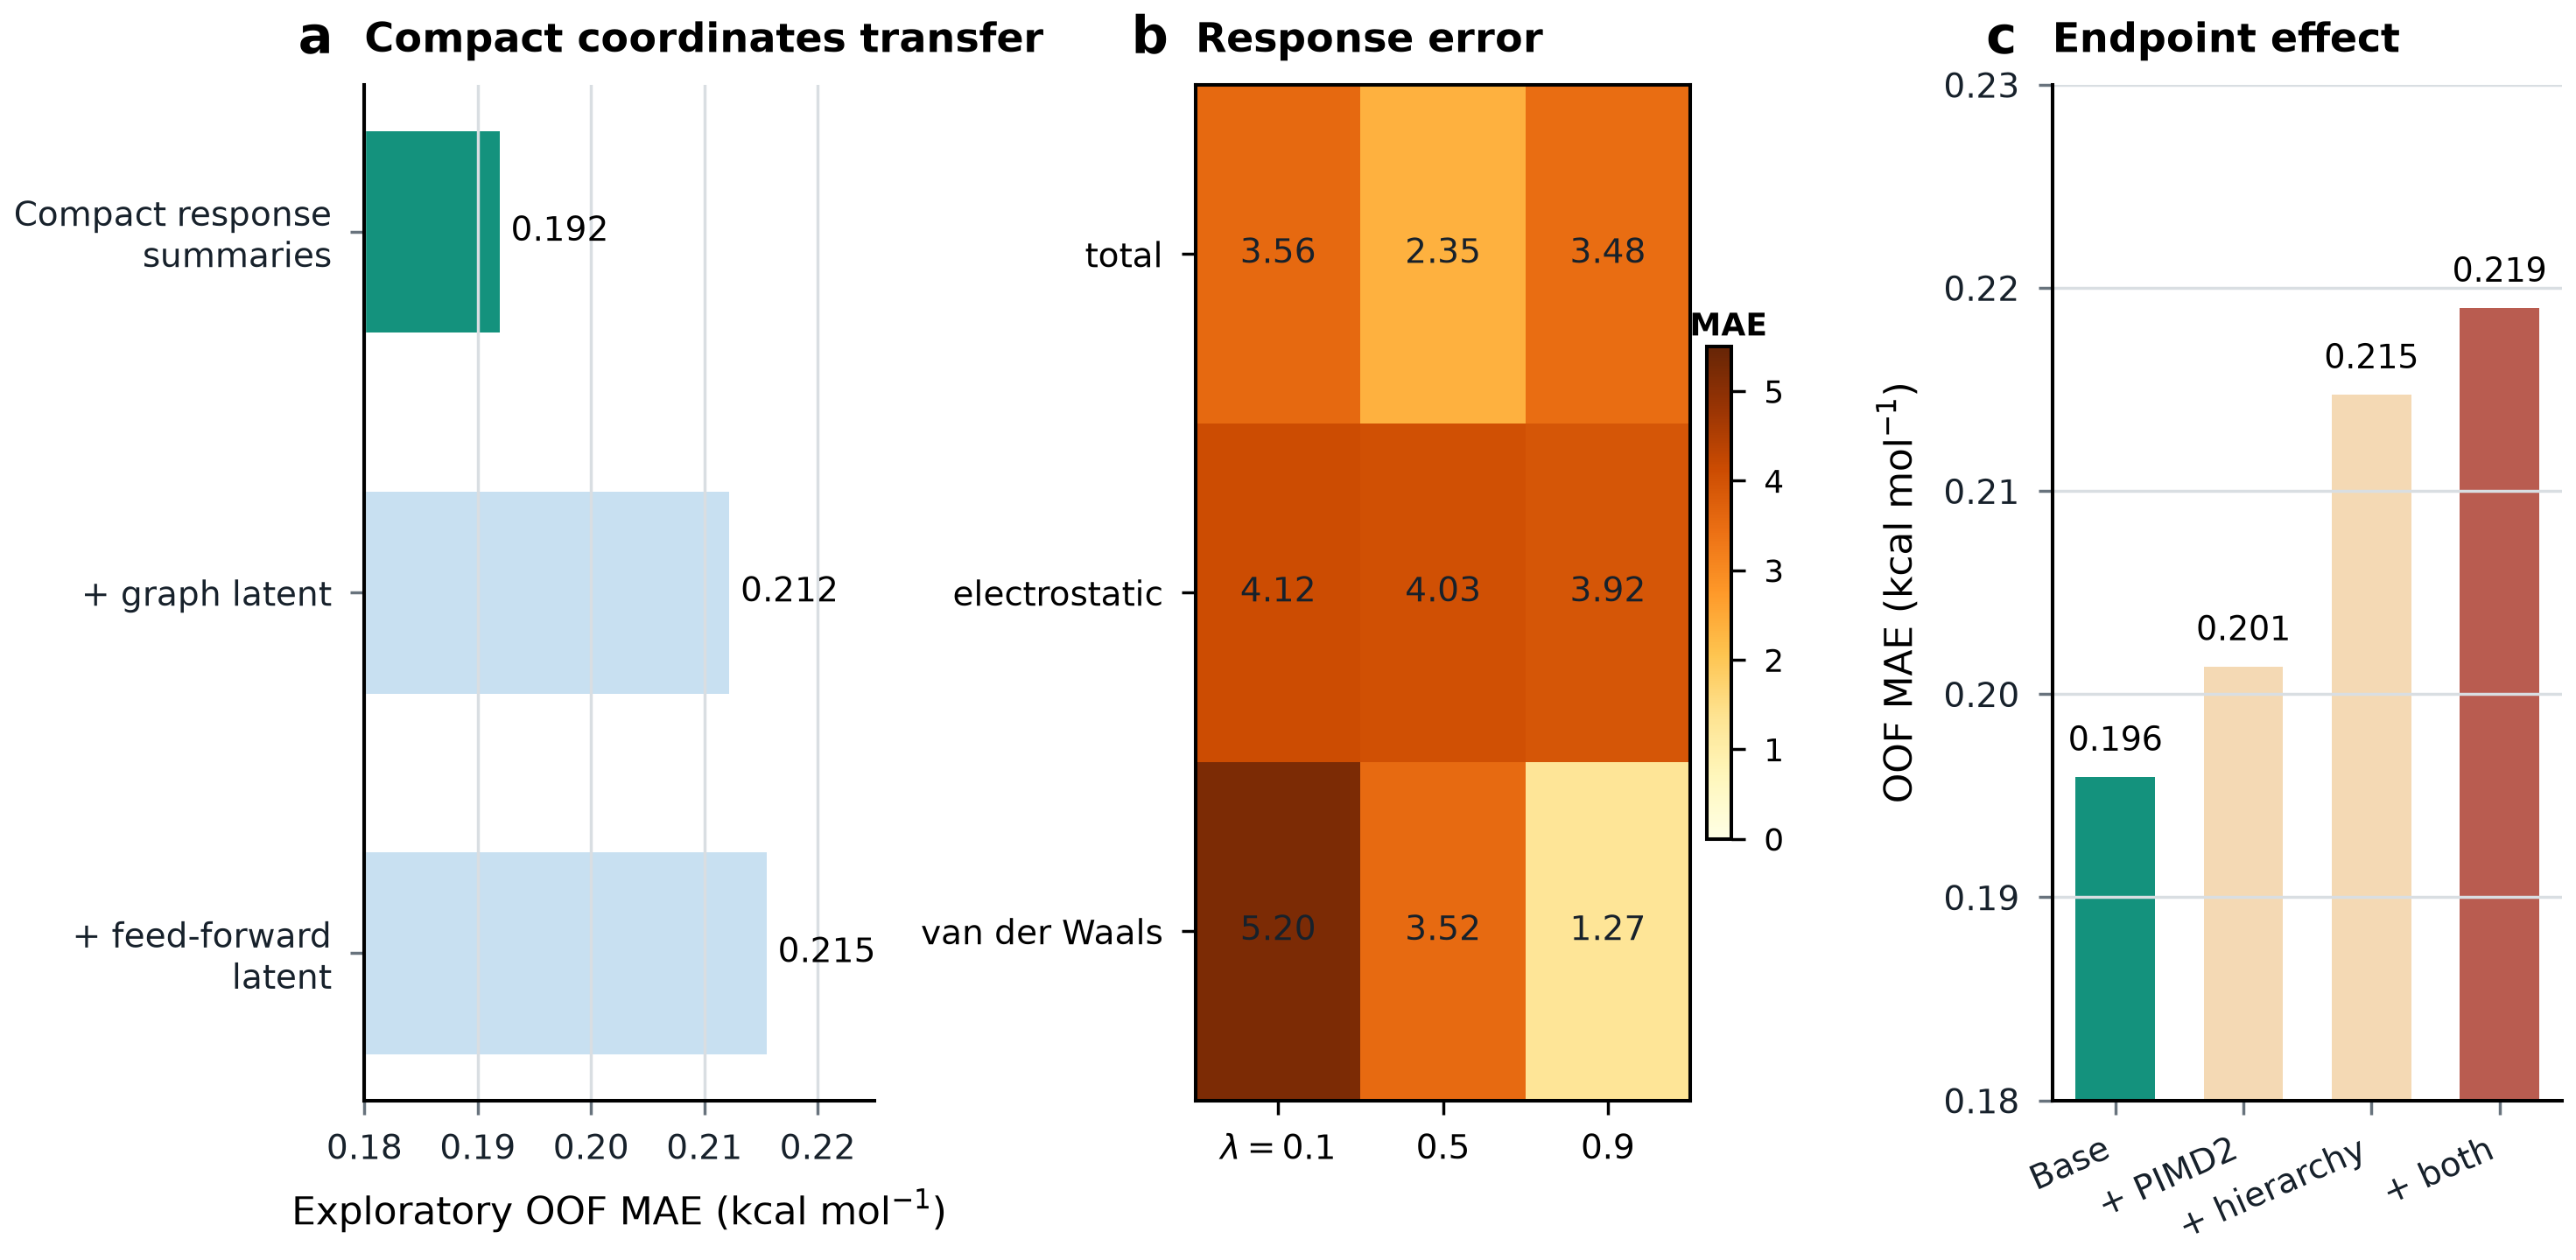
\includegraphics[width=\linewidth]{assets/fig4_frontier.png}
\caption{\textbf{Transfer is limited by structure-to-response accuracy.}
\textbf{a}, Compact ConfSolv summaries versus latent coordinates from the same source.
\textbf{b}, OOF errors of predicted PIMD2 response components. \textbf{c}, Their
endpoint consequences. The negative result motivates the transfer condition; none of
these PIMD-derived blocks enters the final model.}
\label{fig:frontier}
\end{figure}

Together the positive and negative experiments suggest a three-part condition. A
physical response must be relevant to the endpoint, predictable from the representation
available at deployment, and non-redundant with other inputs. Higher-fidelity physics
can be less useful than a coarser coordinate if sparse data make its response
unrecoverable. The transferable object is not ``simulation'' in the abstract, but an
aligned response that survives structure prediction.

\section{What is gained operationally?}

The computational saving is structural rather than a claim about a particular GPU
kernel. A physical calculation is paid for while constructing a teacher source, then
amortized across later queries through the learned response map. On the release host,
the complete CPU pipeline has a warm median of \WarmSingleSeconds{}~s for one
molecule and \BatchSeconds{}~s for a batch of 32
(\BatchPerMoleculeSeconds{}~s per molecule). This is not a millisecond predictor, but
it removes trajectory generation, equilibration, coupling-window sampling, and PIMD
replicas that otherwise recur for each solute. Comparisons with a published 15-window
PIMD8 workload therefore concern total workflow, not same-hardware kernel speed.

The explicit response bottleneck offers a second operational benefit: it identifies
where new computation is valuable. Adding more experimental endpoint labels tests
only the last mapping. Adding source calculations improves a response teacher and can
benefit every endpoint that consumes that coordinate. Conversely, the failed PIMD2
experiment says that sparse high-fidelity labels are currently a poor investment for
this interface. A targeted set of roughly 250--500 chemically diverse molecules with
complete $\lambda$-resolved total, electrostatic, polarization, and
dispersion/repulsion response would test whether that source can cross the
structure-predictability threshold.

\section{Discussion and limitations}

SolvAI changes the unit of reuse for physical computation. Rather than spending a
simulation once to predict one molecule, it treats responses collected across many
molecules as supervision for a reusable coordinate system. Matched ablation, shuffled
priors, global chemical separation, zero-ARROW transport, and frozen external
evaluation all point to the same conclusion: predicted solvent response contributes
information beyond ordinary molecular features and endpoint labels.

The claim is narrower than universal hydration prediction. The primary set has 85
neutral small molecules, and five partitions support an accuracy \emph{scale}, not a
guaranteed sub-0.20 threshold. Accuracy degrades under scaffold and functional-family
separation and on the external cohort. The current model is unvalidated for ions,
salts, biomacromolecules, and substantially larger chemistry; it has no calibrated
per-query applicability score. Its experimentally supervised endpoint should not be
described as a replacement for PIMD where mechanistic trajectories, nuclear quantum
observables, or accuracy outside this domain are required.

The negative PIMD2 result is also a constructive boundary. Direct alchemical-response
distillation will require a larger protocol-matched set spanning response curves and
interaction components, not merely more endpoint labels. More generally, a simulator
is a promising teacher when it exposes a compact response that is predictable across
chemistry and complementary to structure. That criterion offers a way to choose which
expensive calculations are worth amortizing into scientific models.

\section{Methods in brief}

The primary reference comprises the 85 neutral ARROW solutes at 298~K. The endpoint
pool contains 1,147 connectivity-resolved FreeSolv/CombiSolv-Exp records and 133
multi-source SoluteML records after benchmark exclusion
\citep{freesolv2017,combisolvexp2022,soluteml2022}. Fifteen response coordinates are
predicted by six frozen artifact families: CHEMELEON-initialized D-MPNNs for
CombiSolv-QM and MolSolv \citep{chemprop2019}, ExtraTrees models for Abraham and
corrected OpenFF/GBn2 targets \citep{extratrees2006}, and LightGBM models for six
ConfSolv summaries. The endpoint averages three 360-tree ExtraTrees pipelines. The
matched structure-only model removes only the response columns.

The main protocol uses a frozen five-fold partition, followed by five complete
partitions. Block shuffling preserves covariance among the 15 priors. Chemical
separation is applied to the complete supervised pool using deterministic functional
families, Bemis--Murcko scaffolds, Taylor--Butina clusters, or maximum Morgan
similarity. MAE in kcal~mol$^{-1}$ is primary; all comparisons are paired by molecule.
Percentile intervals use 100,000 bootstrap resamples with a predeclared seed. The
external cohort is never used for teacher, feature, threshold, or endpoint selection.
Appendix Secs.~S1--S15 provide full source processing, model settings, identity audit,
fold assignments, sensitivity analyses, tables, runtime, hashes, and molecule-level
results.

Available ARROW outer-training labels receive weight 3 and external endpoint rows
weight 1 in the frozen protocol. A one-factor sensitivity changing only this weight
to 1 leaves the contrast essentially unchanged: \WeightOneStructureMAE{} for
structure only and \WeightOneSolvAIMAE{}~kcal~mol$^{-1}$ for SolvAI, with paired
change \WeightOneDelta{} and a 95\% interval from \WeightOneCILow{} to
\WeightOneCIHigh{}. The all-data deployment artifact is refitted only after evaluation
is frozen and is never used to report paper accuracy. Its SMILES canonicalization does
not imply invariance to tautomer, protonation, or salt form.

The external labels are derived from original-measurement Henry-law records at
298.15~K using $K_c=H_s^{cp}RT$ and
$\Delta G_{\mathrm{hyd}}=-RT\ln K_c$, with 1~M ideal-gas and 1~M
ideal-dilute aqueous standard states. Qualification requires a connected neutral
solute, supported elements, compatible target metadata, and no standardized identity
equivalent in the endpoint pool. One independently documented
name--registry--structure conflict is excluded before evaluation, leaving the 220
reported molecules. No external label participates in fitting, feature choice,
thresholding, or model selection.

\section*{Data and code availability}
An anonymized artifact containing benchmark records, held-out predictions, source
manifests, split assignments, audit tables, frozen inference artifacts, and
reproduction scripts will accompany the submission. Third-party datasets are
referenced by immutable identifiers and hashes where redistribution is restricted.
The public repository address is omitted during double-blind review.

\clearpage
\bibliographystyle{plainnat}
\bibliography{../references}

\clearpage
\nolinenumbers
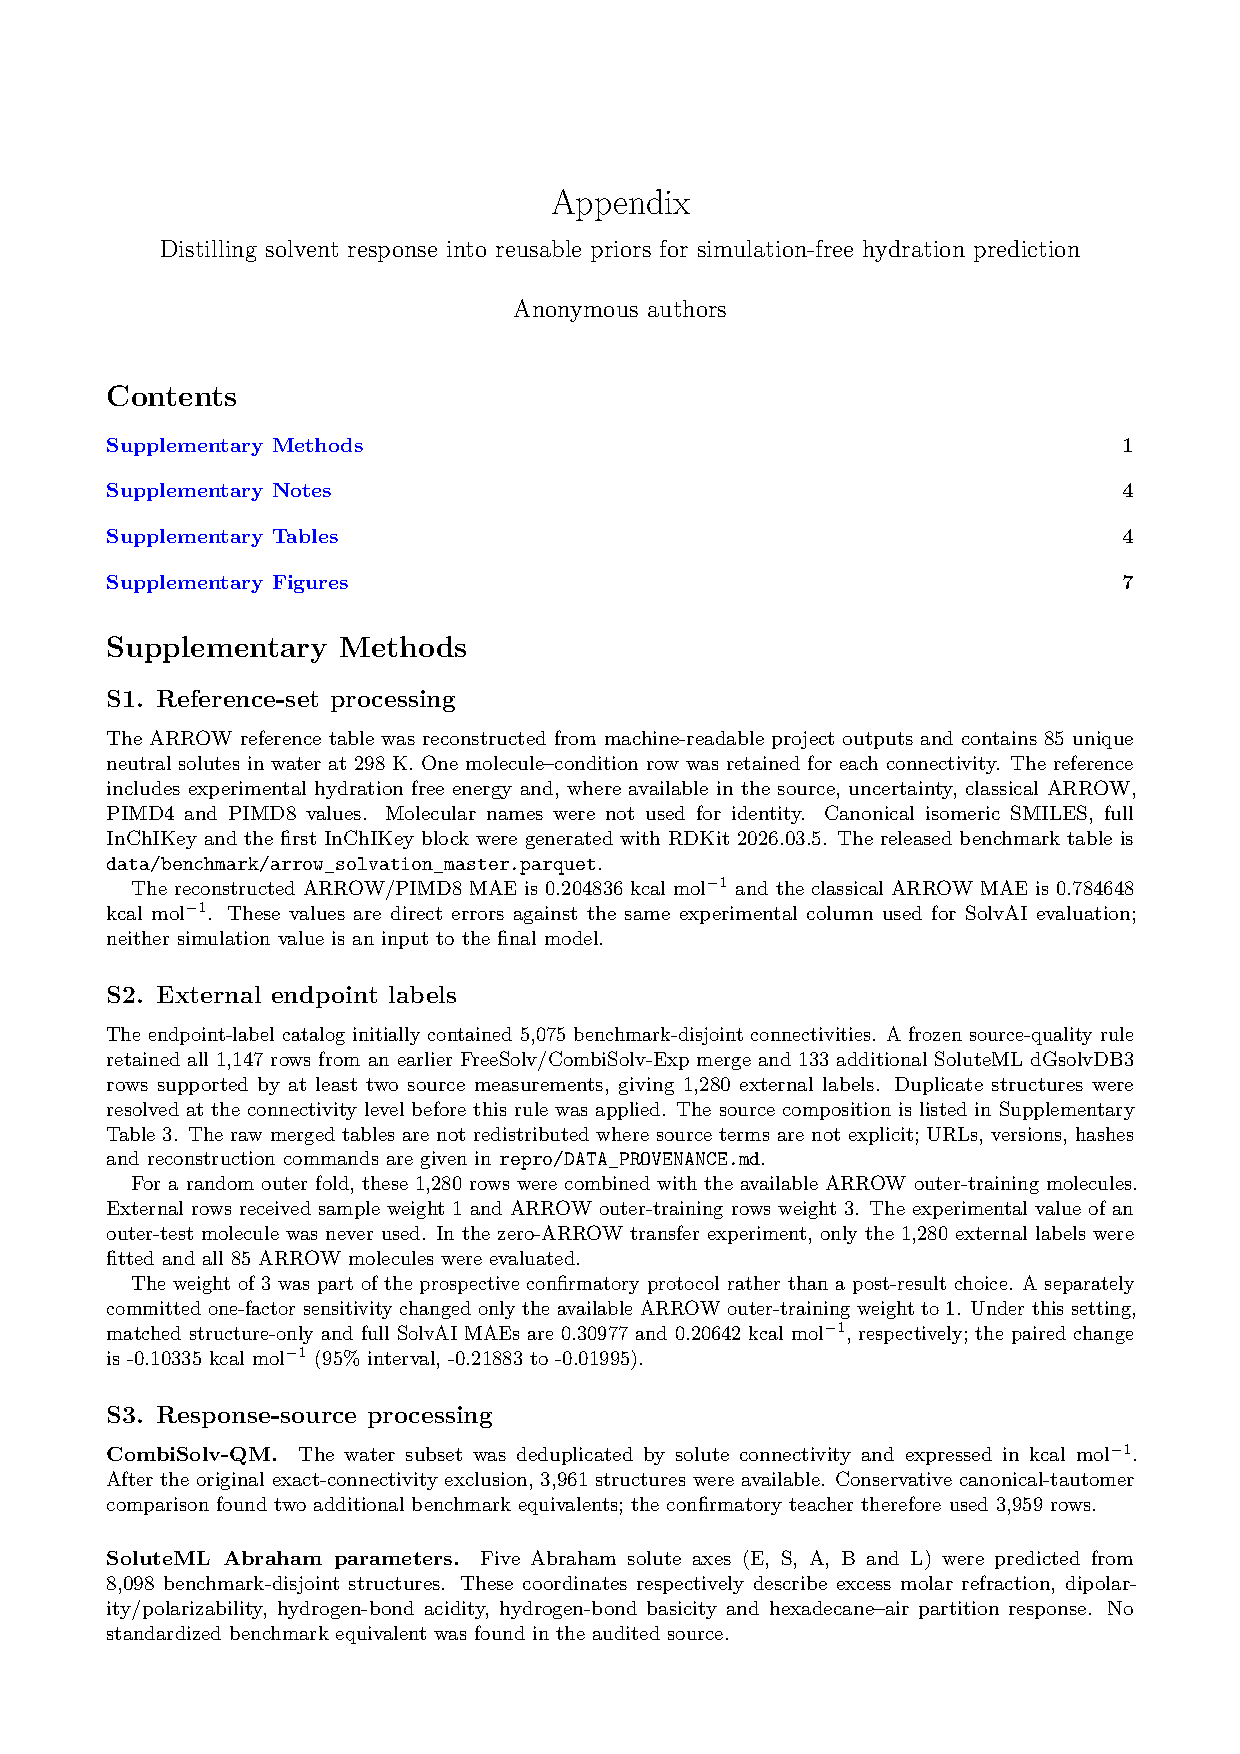
\includepdf[pages=-,pagecommand={\thispagestyle{plain}}]{appendix.pdf}
\linenumbers

\clearpage
\section*{SIMBIOCHEM Submission Checklist}
\begin{enumerate}
\item {\bf Claims}
  \item[] Question: Do the main claims in the abstract and introduction accurately
  reflect the paper's contributions and scope?
  \item[] Answer: \answerYes{}
  \item[] Justification: The abstract and introduction describe the matched
  response-layer contrast and distinguish ARROW-85 accuracy from external-cohort
  transfer.

\item {\bf Limitations}
  \item[] Question: Does the paper discuss the limitations of the work?
  \item[] Answer: \answerYes{}
  \item[] Justification: Section 5 states the molecular domain, external errors,
  missing applicability calibration, and the distinction from PIMD.

\item {\bf AI / LLM disclosure} \emph{(important)}
  \item[] Question: Does the paper disclose any use of AI/LLMs in the research or
  writing (e.g., ideation, code generation, data processing, drafting), in line with
  the NeurIPS LLM policy?
  \item[] Answer: \answerYes{}
  \item[] Justification: Generative AI assisted with adapting and editing the
  manuscript for the workshop format. The authors reviewed the complete text and
  remain responsible for its correctness, originality, and integrity; AI assistance
  did not generate the scientific measurements reported here.

\item {\bf Research integrity \& originality}
  \item[] Question: Do you confirm that this is an original submission---not a
  duplicate or lightly tweaked resubmission, nor one of multiple versions of the same
  work submitted to this workshop---and that you comply with research-integrity
  guidelines?
  \item[] Answer: \answerYes{}
  \item[] Justification: This submission reports the distinct SolvAI response-prior
  study and is not a second version of another submission to this workshop.

\item {\bf Reproducibility} \emph{(optional)}
  \item[] Question: Where applicable, does the paper provide enough information
  (data, code, settings) to reproduce the main results?
  \item[] Answer: \answerYes{}
  \item[] Justification: The appendix records data provenance, identity controls,
  models, folds, statistical procedures, and hashes; an anonymized artifact will
  provide frozen predictions and reproduction scripts.
\end{enumerate}


\end{document}
